\chapter{Technical Background}
\label{sec:tech-background}
Understanding the design and implementation of the windowing system presented in this thesis requires understanding of some technical, domain-specific concepts which may be outside the knowledge base of some readers, so this section is included to consolidate and summarize these concepts. An in-depth discussion of most of these concepts is well outside the scope of this thesis, but references to more detailed explanations are provided where possible. No novel material is presented here, and readers familiar with computer graphics, open-source windowing systems, and the way humans perceive three dimensional space could certainly skip this section altogether.

\section{Computer Graphics}
\label{sec:graphics-pipeline}
The demands of computer graphics applications are fundamentally very different from many other applications, and this has led to the development of specialized hardware coprocessors for accelerating these types of applications called Graphics Processing Units (GPUs). Modern GPUs are programmable computers, much like the CPUs that control them, but they are massively parallel and every aspect of their design is oriented toward exceptionally high data throughput. GPUs are designed to execute a single program on many similar pieces of data in no particular order, making them well suited for computer graphics applications (where a substantial portion of the computational load lies in transforming vertices and shading pixels), as well as many other problems which map well onto the Single Program Multiple Data paradigm. Depending on the GPU manufacturer access to this hardware may be possible through several API’s, but for graphics applications on open source systems the API of choice is OpenGL.
		
OpenGL organizes access to graphics hardware around a data pipeline commonly referred to as ‘The Graphics Pipeline’, and while a detailed description of this pipeline is certainly beyond the scope of this thesis, some of its stages are very important to the design of the windowing system here, so a brief overview is included. Readers seeking further explanation are directed to \cite{graphics-intro} for a good introductory overview of the modern graphics pipeline and \cite{trip-through-pipeline} for a very good and very in-depth discussion of its function. The modern graphics pipeline is complex, and many datapaths exist, but for the scope of this explanation we will focus on the primary datapath illustrated in Figure~\ref{fig:graphics-pipeline}.

\begin{figure}[ht!]
\centering
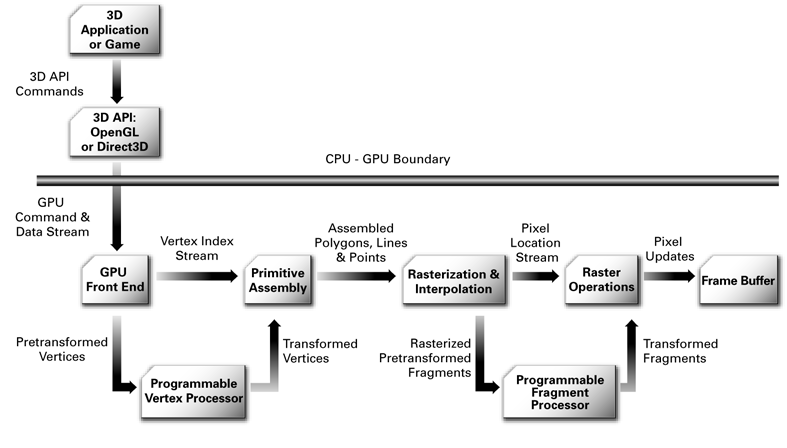
\includegraphics[width=1.0\textwidth]{images/graphics-pipeline.png}
\caption{The basic structure of the graphics pipeline. Note the vertex processor, rasterizer, fragment processor, and termination in a frame buffer. Image taken from  \protect\cite{pipeline-image-ref}}
\label{fig:graphics-pipeline}
\end{figure}


\subsection{The Vertex Transformation}
\label{sec:vertex-transform}
In this datapath, incoming geometry is first transformed in the vertex processor from the space in which it defined into the space in which it is projected onto the 2D output surface. This vertex transformation, shown in Figure~\ref{fig:vertex-transformation} is represented as the composition of several linear transformation matrices in a homogeneous coordinate space, which, being linear transformations, can be applied to the vertices in a sequence or as a composite transform computed as the outer product of the component matrices. Though in principle any number of transformations can compose this composite vertex transformation, it is typically thought of as being composed of three principal transformations. 

\begin{figure}[ht!]
\centering
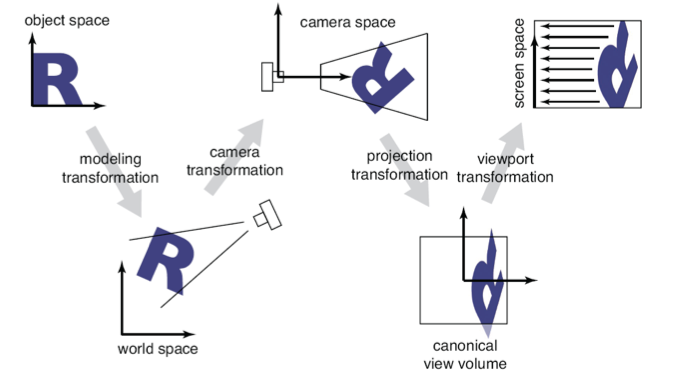
\includegraphics[width=1.0\textwidth]{images/vertex-transformation.png}
\caption{The basic sequence of transformations applied to geometry in the vertex processor. The final transformation in this sequence is applied after the vertex processor and is not part of the composite transformation matrix. Image taken from  \protect\cite{transform-image-ref}}
\label{fig:vertex-transformation}
\end{figure}


The geometry of an object is defined in a space relative to that object, which allows multiple copies of an object placed throughout a scene to share geometry on the GPU. The first transformation, called the ‘modeling transform’ or ‘model matrix’, maps geometry from object space into the space in which the scene is defined, called ‘world space’. The second transformation, called the ‘camera transformation’  or ‘view matrix’, maps geometry from world space into the space of the virtual camera, whose origin is the center of projection of the camera and whose axes are aligned with the camera’s view vectors. This is followed by the projection transformation, which (coupled with a hardware accelerated homogenous divide following output from the vertex processor) maps the vertices into ‘normalized device coordinates’, where all vertices lying inside the view frustum defined by the projection matrix now lie inside the ‘canonical view volume’ reaching from -1.0 to 1.0 along all axes of the new space.
Understanding how these transformations affect the user’s perception of 3D information is important because the synchronization of the matrices that represent them between the client application and the windowing system is the key to correctly compositing 3D clients without needing to do the projection within the windowing system. A simple example is included here to ensure this is clear to all readers.

\subsubsection{A Simple Example: Transformations}

Imagine we have a simple scene containing three objects, a table, a chair, and a room which contains them. Each of these objects has its own model transform, allowing us to move them around independently, but the view and projection matrices are global for all objects, reflecting the idea that there is only one camera. Translating the model matrix of the chair changes where the chair is projected onto the screen, but has no effect on the table or the room, which gives the appearance of the chair moving relative to the room and the table. Translating the view matrix, by contrast, changes how all three objects are projected onto the screen in the same manner. Because humans naturally contextualize the room as a static entity, given their experience with similar structures in reality, this translation gives the viewer the impression of their viewpoint moving through the space containing the objects. Changes to the projection matrix also affect the projection of all three objects, again giving us the impression of changing the properties of the virtual camera. For example, reducing the field of view encoded in the projection matrix affects the resulting image in the same way that a telephoto lense changes the image of reality produced by a real camera. 

\subsection{Rasterization and The Depth Test}
\label{sec:depth-test}
Following output from the vertex processor primitives (like points and lines) are assembled and clipped against the canonical view volume. A final transformation called the ‘viewport transform’ is applied, mapping the X and Y components of the normalized device coordinates into the screen space specified in pixels, and the primitives undergo a process called ‘rasterization’ or ‘scan conversion’, which determines which pixels are covered by the projection of the primitive. A data structure called a ‘fragment’ is generated for each pixel that lies inside the projection of the primitive, and all further stages of the graphics pipeline, including programmable fragment shaders, operate on these fragments. 

At this point we encounter the second concept which is critical to understanding the windowing system presented in this thesis. The vertices (and the primitives assembled from them) are three dimensional, but the screen space in which the fragments are specified is only two dimensional, and in the projection from three dimensions to two some information must be lost. More concretely, it is possible for one object to partially occlude another if it is closer to the camera, and in this case it is necessary that the we draw the closer object in front of the further one. To achieve this behavior the graphics pipeline includes a step called the ‘depth test’ which, depending on the behavior of the fragment shader, takes place either immediately before or immediately after a fragment is run through the fragment processor.

The depth test operates on a two dimensional scalar buffer called the ‘depth buffer’ attached to the active frame buffer which is of the same dimensions as the color buffer being drawn into. The depth of each fragment (the Z component of its position in the projection space) is compared to the depth currently stored in the depth buffer at the XY position of the fragment in question. If the depth of the current fragment is closer than the current contents of the depth buffer the current fragment is drawn, otherwise it is discarded. This guarantees that the closest fragment at a given screen position always determines the color at that position regardless of how many other fragments are drawn to the same screen position or in what order they are drawn. 
The depth buffer is critical to the function of the windowing system presented in this thesis because it can be used to composite the output of 3D applications in 3D using only 2D buffers in the same way that it is used to composite 3D primitives in the normal graphics pipeline (using the same hardware depth test no less), which allows a 3D windowing system to be built on top of windowing infrastructure designed to pass only 2D buffers from applications to the windowing system, and allows applications to use graphics API’s designed around the idea that applications control every aspect of how their 3D content is drawn down to the coloring of the pixels.
Frame Buffers

The termination of the graphics pipeline datapath is a frame buffer. The frame buffer itself is not actually a buffer, but rather a collection of handles for different kinds of buffers, like color buffers or depth buffers, to which actual buffers can be attached. While applications typically render to the ‘default framebuffer’, which represents their actual output to the windowing system (or, in the case of the windowing system, the output to the display), it is also possible for applications to create off-screen frame buffers called Frame Buffer Objects (FBOs) in order to perform multiple rendering passes. This concept is used extensively in the implementation of the windowing system presented here. 

\section{Human Perception of Three Dimensions}
\label{sec:depth-perception}

An important part of this thesis, and computer graphics in general, is exploiting the way that humans perceive three dimensional space to give them the illusion of 3D structure with 2D images. This may appear simple at a high level, since the human eye can only sense two dimensional images, but the way that humans use these 2D images to reconstruct the 3D structure of reality is extremely sophisticated and this makes the process of generating a compelling illusion much more complicated. Humans rely on a number of behaviors in the way the 3D structure of reality is projected to two dimensions by their eyes, called ‘depth cues’, to inform their understanding of the 3D structure of the scene they are observing.
	
There are many of these depth cues and, to the authors knowledge, no graphical system is capable of presenting all of them consistently to the user, but it is important for proper 3D perception that those cues which are present are consistent with one another and consistent between different parts of the scene. Because the windowing system presented in this thesis attempts to combine the output from different 3D applications into a cohesive 3D scene while still allowing these applications to control the projection of their 3D content to 2D, the synchronization of the parameters which control these depth cues between the compositor and the client applications is an important part of the work presented here. A brief overview of some of the relevant depth cues in included here to ensure all readers are familiar with the mechanism that enables them, as this is needed to understand the way the windowing system presented here creates the illusion of a consistent 3D scene composed of multiple 3D clients. The focus of this section is on depth cues which are handled by the windowing system presented here, for a more comprehensive and in depth discussion of depth cues in general, readers are directed to \cite{depth-cues}.

\subsection{Motion Parallax and Stereopsis}
\label{sec:motion-parallax-and-stereopsis}

A key property of three dimensional space that allows us to perceive its structure from two dimensional images is that imaging the same 3D scene from different points in space results in different 2D images. Should this not be immediately apparent to the reader they are invited to hold their hand at arms length, move their head around, and observe how the portion of the scene which is occluded by their hand changes in response to the movement of their head. This effect, called ‘parallax’ forms the base of two very important and closely related depth cues: motion parallax (the change in projection based on the position and orientation of the users head), and stereo parallax or ‘stereopsis’ (the difference in the projection between the user’s eyes due to their slightly different location in space). On the hardware side, achieving the former requires that the system actively measure the position of the user’s head (called ‘head tracking’), and achieving the latter requires that the system be able to display a different image to each of the user’s eyes (making it a so called ‘stereo display’), and these two capabilities together form the requirements set forth in Section~\ref{sec:3d-display}) for and ‘immersive 3D display’. On the software side, the position of the virtual camera is controlled by the content of the view matrix (as explained in Section~\ref{sec:vertex-transform})) , and so stereopsis requires that there be a separate view matrix for each eye (and that the scene is projected separately for each of these matrices) and motion parallax requires that these matrices change in response to changes in the user’s measured head transform.

Maintaining consistency is the effects of stereopsis and motion parallax between the compositor and all of its 3D client applications requires that all entities involved projecting 3D geometry do so with the same view matrices for each eye, and so an important part of the Wayland protocol extensions presented here is providing 3D clients with up to date view matrices for each eye before each frame is drawn, and giving the clients a mechanism for providing the compositor with different output for each of the user’s eyes.

\subsection{Relative Size}

Relative size refers to the change in the size of the projection of an object as it’s distance from the viewer changes, with objects appearing smaller to the viewer as they recede further into the distance. This behavior is achieved with, and is the primary purpose of, the projection matrix discussed in Section {The Vertex Transform}, which maps the frustum of space visible from the camera position (called the view frustum) onto the cubic region of space defined by the normalized device coordinates. Because the portion of the view frustum that is closer to the camera position is narrower than the portion which is further away, the process of mapping it into normalized device coordinates compresses geometry in the view frustum more the further it is from the camera position, making this geometry smaller the further it is from the camera, creating the illusion of relative size. In order to maintain the consistency in the relative size cue between all of the client applications and the compositor, it is necessary that all parts of the windowing system doing 3D projection do so using the same projection matrix, which is an important part of the display server protocol extensions presented here.

\subsection{Occlusion}

Another important, and familiar, aspect of three dimensional space is that when imaged onto a two dimensional plane, portions of the scene which are closer to the camera can hide, or ‘occlude’, portions that are further away. This gives us a powerful depth cue, because the occlusion of an object by another immediately tells us that the second object is closer, and the portion of the object that is occluded gives us even more detailed information about their spatial relation. As explained in Section {Rasterization and The Depth Test}, this behavior is achieved in the graphics pipeline by maintaining a 2D buffer containing the depth of each pixel, and only drawing a new pixel if it closer than the contents of the depth buffer. While this technique is both efficient and effective, using it to composite 3D content from multiple clients requires that the compositor have access to not only its own depth buffer, but also the depth buffers of all the 3D clients, and so providing a mechanism that allows this is an important part of the Wayland extensions presented here. 

\section{Open Source Windowing Systems}

Though the basic concept of windowing systems pervades all graphical operating systems, there are some architectural details of the windowing systems used in open source operating systems which are relevant to the windowing system presented in this thesis. This discussion will focus on X, which has been the predominant Linux windowing system for almost two decades, and its replacement, Wayland, which forms the foundation of the windowing system presented in this thesis.

\subsection{Basic Architecture}

Wayland, like X, operates on a client-server model, where the clients are the applications needing a graphical interface services (like the ability to create a window and listen for input events), and the server is a program, called a display server, which interfaces directly with the display and input devices and uses them to meet the interface needs of the client applications. The clients   connect to the server through a Unix socket and the two communicate via a protocol called the `display server protocol`. The names X and Wayland both technically refer to the display server protocol itself, and in both cases the protocol is extensible, allowing the windowing system to dynamically meet the needs of graphical systems as they change with technological development. This has largely allowed X to withstand the test of time, although the developers behind Wayland argue that the way X is currently used is so tangential to its original design goals that its function has largely degraded to providing “really bad IPC” \cite{real-story-wayland}. The effort to resolve these problems led to the development of Wayland, which, as the Wayland architecture page states, is most easily understood through comparison with X \cite{wayland}.

\subsection{Wayland and X}

As with the other topics in this section, a thorough discussion of the architectural differences between Wayland and X is both outside the scope of this thesis and largely irrelevant to the windowing system presented here, and interested readers are directed to \cite{wayland} and \cite{real-story-wayland} for more information. However, there is one architectural feature of X which makes it unsuitable for supporting the windowing system described here.

\begin{figure}[ht!]
\centering
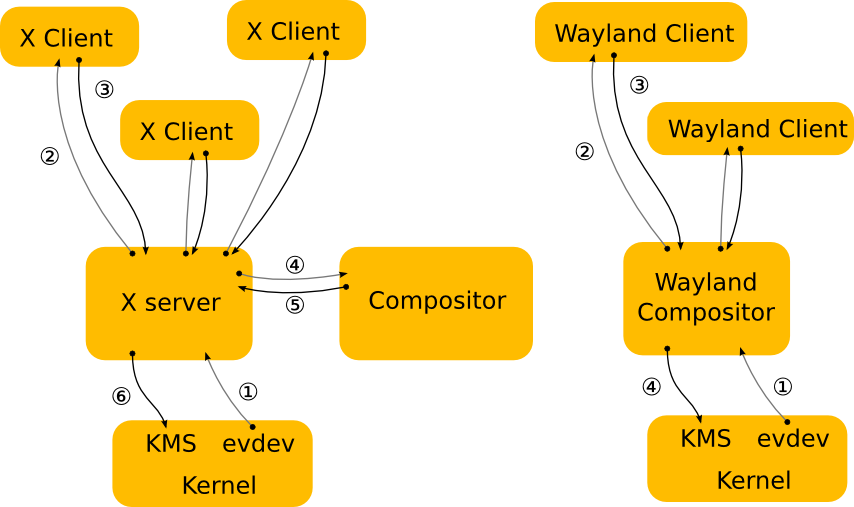
\includegraphics[width=1.0\textwidth]{images/wayland-x-architecture.png}
\caption{High level architecture of the X and Wayland windowing systems. Note that the X compositor is a separate entity from the display server, whereas the Wayland compositor provides the functionality of the display server internally. Images taken from  \protect\cite{wayland}}
\label{fig:wayland-vs-x}
\end{figure}



As illustrated in Figure~\ref{fig:wayland-vs-x}, the high level operation of the two windowing systems is largely the same, and the interface between the kernel and the display server are recycled, allowing Wayland to reuse much of the infrastructure developed to support X. The key difference that is relevant to this thesis, immediately visible in Figure~\ref{fig:wayland-vs-x}, is Wayland’s integration of the display server and the compositor. 

In the X architecture, the compositor is a client, just like the applications, that communicates with the display server over the display server protocol. When clients send their output to the display server it is forwarded to the compositor, which composites the output based on its internal scenegraph of how the windows are laid out (which can, in the case of some compositors like Compiz, contain 3D window transformations), and sends this composited output back to the display server, which then draws it to the display. The key problem here is that the X server has its own internal representation of how the windows are laid out (which is strictly two dimensional), and when it receives input events from the kernel it  determines which window to deliver them to based on the location of the event and its own internal layout of the windows, rather than letting the compositor control the input event redirection. This means that if the compositor applies a 3D transformation to the window, this is not reflected in the X server’s internal window layout and so input events are not redirected to the appropriate client or transformed correctly into the client’s window space, making it essentially impossible to interact with windowed X applications in a meaningful way when they are embedded in a 3D space. 

In the Wayland architecture, by contrast, the compositor and the display server are the same entity and therefore by definition share an internal representation of how the windows are laid out. This allows the compositor to give windows an arbitrary embedding in a 3D space and still deliver input events to the applications driving them in a meaningful way. It also means that input events do not necessarily need to be delivered based on the embedding of the window surface itself, but can be delivered based on the embedding of an arbitrary spatial data structure associated with the surface, which is critical to the way the windowing system presented in this thesis handles 3D applications, since the output is drawn on a 2D surface but the interaction space the user perceives the user perceives for the application is three dimensional.


\subsection{Wayland Display Server Protocol}

The Wayland display server protocol, detailed in \cite{wayland-protocol}, is an asynchronous, object oriented protocol in which the compositor advertises objects which can accept requests from clients and generate events which the clients to which the clients can respond. These objects are either globally defined or contained within a global object, and can have any type defined in the core protocol specification or extensions to this protocol. When an object is created, all clients are notified via a creation event, and when a client connects it receives such a creation event for every global object which is already globally defined.

The protocol is defined in a set of Extensible Markup Language (XML) files from which language bindings for a specific programming language can be generated dynamically, allowing clients and compositors to be written in any language and still communicate with one another via the Wayland protocol. A program which generates C language bindings from XML protocol definitions, called wayland-scanner, is provided by the Wayland developers. The protocol can be extended by simply defining new object types, requests, and events in a separate XML file (or set of files), creating language bindings from these files, and then including these language bindings in the compositor and the clients. Compositors can support extensions not supported by a client without compromising the ability of these clients to communicate with the compositor, which allows compositors to support broad classes of clients without these clients needing to support, or even be aware of, the same set of extensions.

The system presented in this thesis defines a set of extensions to the Wayland protocol which allow it to provide 3D windowing services to clients which support these extensions, while simultaneously fully supporting clients which are designed to interact with traditional, 2D Wayland compositors.

\subsection{EGL}

The Khronos Group EGL Native Platform Interface (EGL) \cite{egl} is an API specified by Khronos Group (who also specify APIs like OpenGL and OpenVG) which `provides mechanisms for creating rendering surfaces onto which client APIs like OpenGL ES and OpenVG can draw, creates graphics contexts for client APIs, and synchronizes drawing by client APIs as well as native platform rendering APIs` \cite{egl}. In the Wayland architecture, EGL allows clients to create a drawing surface on the GPU (essentially region of GPU memory that can be filled with an image with a specific color format), and allows the compositor to access the contents of this surface directly  and use it for hardware accelerated compositing without ever needing to take the contents of the surface off of the GPU. 

While the internal function of EGL has little impact on the design of the system presented here (since EGL is mostly handled by the underlying subsystems on which it it is built), it is important for the reader to understand at a basic level how EGL fits into Wayland, since EGL's inability to give the compositor direct access to the client depth buffer strongly affects the way that client depth buffers and the depth compositing process are handled by the system, as well as the performance of the depth compositing process.